On réalise un oscillateur \{solide $\mathrm{(S)}$, ressort\} en fixant un solide
$\mathrm{(S)}$, de centre d'inertie $G$ et de masse $m$, à l'extrémité d'un
ressort horizontal à spires non jointives, de masse négligeable et de raideur
$K$.

On écarte $\mathrm{(S)}$ de sa position d'équilibre d'une distance $X_{m}$, et
on le libère sans vitesse initiale à l'instant $t_{0}=0$. Le solide
$\mathrm{(S)}$ est animé d'un mouvement de translation rectiligne sinusoïdal
d'équation horaire ${x(t)=\num{5.e-2}\cdot\cos(2\pi\cdot t)~(\unit{\m})}$.

\begin{minipage}{0.64\linewidth}
    \textbf{Données~:} $m=\qty{1}{\kg}$
    \begin{enumerate}[series=x]
        \item Déterminer la valeur de $X_{m}$ et celle de la période propre
              $T_{0}$ des oscillations.
        \item Calculer la valeur de la raideur $K$ (On prend $\pi^{2}=10$).
        \item On choisit l'état où le ressort n'est pas déformé comme état de
              référence de l'énergie potentielle élastique $E_{pe}$, et le plan
              horizontal contenant $G$ comme état de référence de l'énergie
              potentielle de pesanteur $E_{pp}$.
    
              La figure 3 donne les variations de l'énergie cinétique $E_{C}$ du
              solide $\mathrm{(S)}$ en fonction de l'élongation $x$ de $G$.
    \end{enumerate}
\end{minipage}
\hfill
\begin{minipage}{0.34\linewidth}
    \begin{figure}[H]
        \centering
        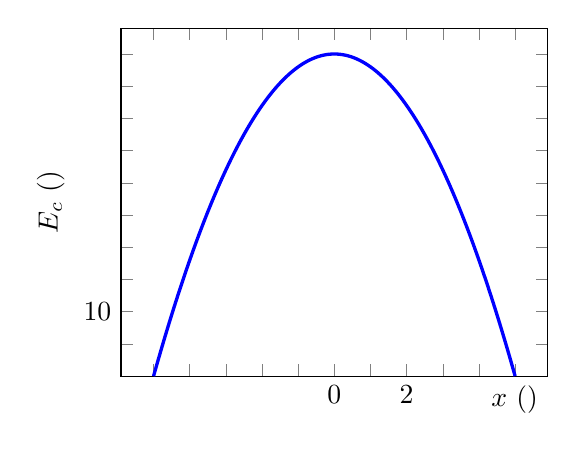
\begin{tikzpicture}
            \def\K{40}
            \def\Xm{0.05}
            \begin{axis}[
                    xmin=-0.059,xmax=0.059,
                    ymin=0,ymax=54,
                    width=7cm,height=6cm,
                    xlabel=$x~(\unit{\cm})$,
                    ylabel=$E_{c}~(\unit{\mJ})$,
                    every axis x label/.append style={
                        at={(1,0)},anchor=north east,
                    },
                    scaled ticks=false,
                    xtick distance=0.01, ytick distance=5,
                    xticklabels={,,,,,,0,,2}, yticklabels={,,,10},
                    minor tick num=0,
                ]
                \addplot[domain=-\Xm:\Xm,samples=200,
                    very thick,blue] {0.5*\K*(\Xm^2-x^2)*1e3};
            \end{axis}
        \end{tikzpicture}
        \caption{}
        \label{fig:2bac_svt_national_2025_rattrapage_phys_ex3_3}
    \end{figure}
\end{minipage}

\begin{enumerate}[resume=x]
    \item[]
    \begin{enumerate}
        \item Justifier que l'énergie mécanique du système se conserve.
        \item Déterminer la valeur de l'énergie potentielle élastique
              $E_{pe}$ lorsque $G$ atteint l'élongation maximale.
        \item Calculer le travail $W(\vec{F})$ de la force exercée par le
              ressort sur le solide $\mathrm{(S)}$, lorsque $G$ passe de
              la position d'élongation $x=X_{m}$ à la position
              d'élongation $x_{0}=0$.
    \end{enumerate}
\end{enumerate}


